\documentclass[a4paper]{article}
\usepackage[utf8]{inputenc}
\usepackage{hyperref} %URLS
\usepackage{graphicx} %graphics
\usepackage[underline=false,rounded corners=false]{pgf-umlsd} %UML Sequence diagrams
\title{Programmiertechniken in der Computerlinguistik III \\ Projektentwurf Gruppenarbeit}
\author{Myriam Truffert,  Raphael Balimann}
\date{2014/10/04}

\begin{document}

\maketitle

\section{Formalia}

\subsection{Beteiligte}

\begin{itemize}
	\item Myriam Truffert (\url{mailto:myriam.truffert@uzh.ch})
	\item Raphael Balimann (\url{mailto:raphael.balimann@uzh.ch})
\end{itemize}

\subsection{Gruppenname (WIP)}

\begin{itemize}
	\item GO
	\item GOàgogo
	\item Tangoschatz
	\item METAgo
\end{itemize}

\section{Motivation}

Über das Internet stellen sich zur Verfügung hilfreichen Ressourcen für Leute, die ihre Sprachkenntnisse vertiefen möchten. Dafür bietet \href{https://www.wiktionary.org/}{Wiktionary} zum Beispiel gratis verschiedenen Details über Wörter (die Herkunft, das Gebrauch, die Synonyme, die Übersetzungen...). Mit \href{http://ankisrs.net/}{Anki} können die Lernende mit selbst vorbereiteten Karten der Wortschatz einüben. (Bei \href{http://www.languagecourse.net/vocabulary-trainer.php}{LanguageCourse} können die Lernende eine bestimmte Sprache und ein bestimmtes Niveau wählen und ihres Wortschatz trainieren.) \href{http://en.pons.com/translate}{Pons}-Verlag bietet bilinguale Online-Wörterbücher für verschiedene Sprachen mit einer Option ``Vokabeltrainer“.  \href{http://jisho.org/}{Jisho} ist auch ein sehr gutes Online-Wörterbuch für Japanisch-Englisch. Als Computerlinguisten wollen wir durch dieses Projekt ein Programm erstellen, damit Lernende den Wortschatz ihre Lieblingsprachen studieren können. Wir möchten alle die Vorteile von die vorher erwähnte Online-Ressourcen für unseres Programm ausnutzen. Ausserdem, die Wörterbücher bilden schon freie Daten, die wie implementieren können. Unsere Ziele sind die Vereinfachung von Wörterbuchzugriff und Vokabularaufbau zu ermöglichen. 
.
\\
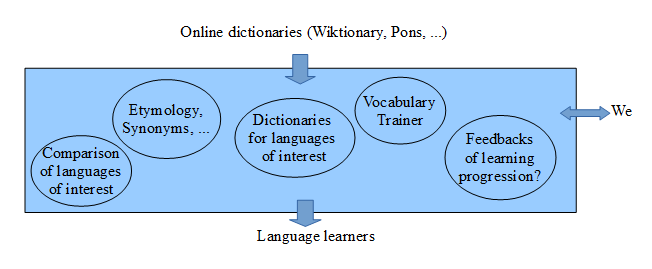
\includegraphics[scale=0.75]{UseCaseUML}
\\

\section{Aufbau des Systems}

\subsection{Komponenten}

\begin{itemize}
	\item Eingabeformular (Webdienst)
	\item Erkennung der Sprache
	\item Vereinheitlichung der Anfragen (Skript auf Server)
	\item Abfragen an Drittservices (Skript auf Server)
	\item Ausgabe der Ergebnisse als Tabelle (Webdienst)
	\item Manipulation der Ergebnistabelle (Webdienst)
	\item Ausgabe der Ergebnisse als strukturierte Daten
	\item Fallback auf externe SMT-Services (z.B. MyMemory)
	\item (Skripte für Import in lokale Lerndatenbanken der User)
	\item Ausgabe der strukturierten Daten als XML oder CSV
\end{itemize}

\subsection{Komponenten}

\begin{itemize}
	\item Webserver
	\item API-Zugriff auf SMT-Services (z.B. MyMemory)
\end{itemize}

\subsection{Funktionsweise}
%UML-Sequence-Diagramm
\begin{sequencediagram}
\newinst{u}{User}
\newinst{w}{Webservice}
\newinst{z}{Server (UZH)}
\newinst{i}{interne Services}
\newinst{e}{externe Services}
\begin{call}{u}{get translations(input)}{w}{return table}
\begin{call}{w}{get translations(input)}{z}{return table}
\begin{call}{z}{get language(input)}{e}{return language}
\end{call}
\begin{call}{z}{get tokens(input)}{i}{return tokens}
\end{call}
\begin{call}{z}{get translation(tokens)}{e}{return translation}
\end{call}
\begin{call}{z}{get normalized(translation)}{i}{return normalized}
\end{call}
\begin{call}{z}{get table(normalized)}{i}{return table}
\end{call}
\end{call}
\end{call}
\begin{call}{u}{get data(selection)}{w}{return data}
\begin{call}{w}{get data(selection)}{z}{return data}
\begin{call}{z}{get data(selection)}{i}{return data}
\end{call}
\end{call}
\end{call}

\end{sequencediagram}

%\begin{enumerate}
%	\item User-Server: getTranslations(text)
%	\item Server: getTokens(text) - fetchTokens(tokenizedText)
%	\item Server-(3rd)Server: getLanguage(tokenizedText)
%	\item Server-3rdServer: getTranslation(tokenizedText)
%	\item 3rdServer-Server: fetchTranslation(translatedText)
%	\item Server: normalizeResults([translatedText1, ..., TranslatedTextN)
%	\item Server-User: fetchTranslations(textTable)
%	\item User-Server: getData(language, format, parameters)
%	\item Server: transformResults(textTable)
%	\item Server-User: fetchData(structuredData)
%\end{enumerate}

\subsection{offene Fragen}

\begin{itemize}
	\item API für Wörterbücher
	\item API für (S)MT
	\item Textsupport (Unicode)
	\item zu unterstützende Textformate
	\item zu unterstützende Programme (z.B. Anki als offenes Spaced-Repetition-System mit Möglichkeiten für Add-Ons)
\end{itemize}

\section{Projektplan}

Bis am 15.10.2014 (Myriam):

\begin{itemize}
	\item Einrichtung Server UZH
	\item Interface für Eingabeformular
	\item Normalisierungs-Skript für User-Anfragen
\end{itemize}

Bis am 29.10.2014 (Raphael):
\begin{itemize}
	\item Spracherkennungs-(Anfrage)-Skript
	\item API-Anfrage-Skripts für jeweilige Web-Services
	\item Normalisierungs-Skript für API-Resultate
\end{itemize}

Bis am 12.11. 2014 (Myriam)
\begin{itemize}
	\item Fallback-Anfrage-Skript
	\item Darstellung als Tabelle (Design und Skripting)
	\item Interface für Tabellenmanipulation
\end{itemize}

Bis am 26.11.2014 (Raphael)
\begin{itemize}	
	\item Konversions-Skripte für Dateiformate
	\item (Add-Ons für externe Programme)
\end{itemize}

\end{document}
